\documentclass{article}
\usepackage{ams math,amssymb,graphicx,listings}
\usepackage{fullpage}
\begin{document}
UPC Study Group Homework - Performance Analysis\\
For these experiments, wen will use the CrayPat utility and therefore need to run on one of NERSC's Cray systems.  We will be using Hopper.  This is an introduction to profiling your code and is by no means comprehensive.  However, as we hopefully discussed during the study group, it's not always clear which parts of your code may be causing performance bottlenecks.  This is probably particularly true when making use of 3rd party software that may or may not be optimized.  In order to figure out where your pipelines are running into trouble, you can make use of profiling tools.  In this document I'll run through a brief example and then your assignment is to do some experiments on your own.  \\

I recommend using the code phyldog (bioinformatics related software) for this since it is an MPI code we have already built on Hopper, but feel free to build your own, just remember to move the executable to SCRATCH space before running your experiments.   

\section{Motivation}


\section{Using CrayPat}
 
 There are some basic steps for using CrayPat 
 \begin{enumerate}
 \item Load the perftools modulefile
 \item Build the application and keep the .o files
 \item Instrument the application using \verb+pat_build+
 \item Run the instrumented executable to get a performance data file (".xf file")
 \item Run \verb+pat_report+ on the data file to view the results
 \end{enumerate}
 
 \subsection{Sampling}
Sampling (sometimes called "asynchronous") means the software will sample the program counter (PC) or the call stack at given time intervals or when specified counter overflows.  The program counter provides information about the state of your application at a given time

The program counter (PC), commonly called the instruction pointer (IP) in Intel x86 and Itanium microprocessors, and sometimes called the instruction address register (IAR)[1] or just part of the instruction sequencer,[2] is a processor register that indicates where a computer is in its program sequence.
In most processors, PC is incremented after fetching an instruction, and holds the memory address of (�points to�) the next instruction that would be executed. (In a processor where the incrementation precedes the fetch, PC points to the current instruction being executed.)

More information on how the CPU works can be found in any number of good textbooks and is beyond the scope of this homework assignment. 

The default experiment type is to sample the PC at a time interval (i.e., \verb+samp_pc_time+). There are other sampling experiment types available.  The type can be set by the environment variable \verb+PAT_RT_EXPERIMENT+ (see the \verb+intro_craypat+ man page)
 
\subsection{Tracing}
Tracing Experiments

\verb+pat_build+ also can instrument an executable to trace calls to user-defined functions and Cray-provided library functions (e.g., MPI functions). Again, to generate an instrumented executable, one needs to load the perftools module first, and then compile and link the binary in separate steps.
 
\subsection{Automatic Program Analysis}
A sampling experiment runs with little overhead, but a detailed tracing experiment typically comes with large overhead, especially as you increase the number of nodes or cores used for the experiment.  Therefore, it's a good strategy to first run a sampling experiment to identify routines that would benefit from a full tracing experiment.  Once the routines are identified, the executable can be instrumented and the tracing experiments can be performed.  This should reduce the overall time needed to run the profiling experiments.  

CrayPat's Automatic Program Analysis (APA) feature provides an easy way to determine the routines that should be instrumented for a full trace.  The executable is instrumented for a sampling experiment and when the binary is executed, it generates an ASCII text file that contains CrayPat's suggestion for \verb+pat_build+ tracing options.  These options can be used to re-instrument the executable for detailed tracing experiments.

\section{Perftools examples and questions}
To give an idea of how this all works, we'll make use of the code in \verb+/scratch/scratchdirs/kmfagnan/perftools/+ on Hopper.  These examples were developed for a tutorial given by NERSC consultants a year and a half ago.  The code is very simple to analyze, making it a great starting point for understanding the basics of profiling.  For extra credit, you have the option to profile a code that we just built and started using on Hopper - Phyldog, OR any other code of your choosing.  We will be discussing this again in the context of how to profile your codes on Genepool, but it's going to take some more time. 


You might want to copy \verb+/scratch/scratchdirs/kmfagnan/perftools.tar+ to your own scratch directory. 

\subsection{Serial example, heap size}
For this first question, we will just be looking at the basic output generated with no options to \verb+pat_build+ and we will check to be sure that basic statistics like the memory HiWater mark are being reported properly.

\begin{lstlisting}
> module load perftools
> ftn -c jacobi_serial.f90
> ftn -o jacobi_serial
  jacobi_serial.o
> pat_build jacobi_serial
\end{lstlisting}

Now, run the executable \verb?jacobi_serial+pat? in a batch job (available as runit in the /perftools/sampling directory).

What do we see when we run
\begin{lstlisting}
> pat_report jacobi_serial+pat+5511-2558sot.xf
\end{lstlisting}

There are three tables of data that are getting reported, along with legends that provide basic information on what is contained in the tables.
\begin{center}
\begin{figure}[htbp]
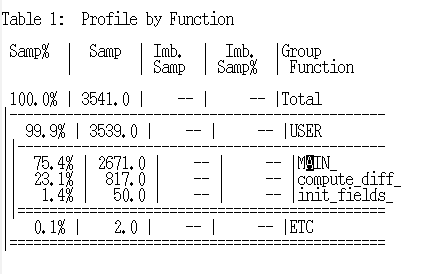
\includegraphics[scale=.5]{images/heap_exp_table1.png}\\
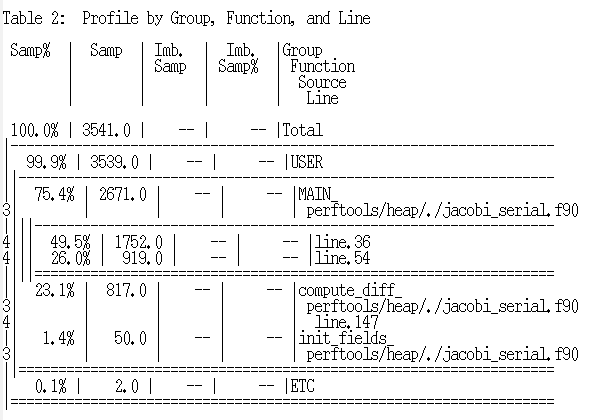
\includegraphics[scale=.5]{images/heap_exp_table2.png}\\
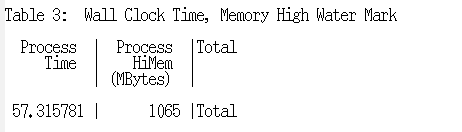
\includegraphics[scale=.5]{images/heap_exp_table3.png}
\caption{Tables from the basic heap HiWater mark experiment.  }
\label{fig:heap}
\end{figure}
\end{center}

If we take a look at the information in the tables in Figure \ref{fig:heap}, we notice a few things.  In Table 1 information is reported for each function that has been called and the percent time spent in each routine is reported.  This gives us an idea of which routines in the code are consuming the most resources and would be good to focus on for code optimization.  

The second table breaks down the same basic information and points out specific lines where the majority of the calculation time is being spent by function \verb+(main, compute_diff, init_fields)+.  For the MAIN function, if we take a look at the code, specifically line 36,
\begin{lstlisting}
      do i=1,n-1
        utmp = 0.25 * ( u(i+1,j) + u(i-1,j) &
             + u(i,j+1) + u(i,j-1) &
             - h * h * f(i,j) )
        unew(i,j) = omega * utmp + (1. - omega) * u(i,j)
      enddo
\end{lstlisting}
we see that this is the start of an innermost for-loop and it makes sense that this would be where the code spends a lot of time.  Then the next line where a lot is going on is line 54,
\begin{lstlisting}
!   Make the new value the old value for the next iteration.

    u(:,:) = unew(:,:)
\end{lstlisting}
where vector assignment is happening.  

In the

The third and fourth column indicate load imbalance and will be useful in the MPI and OpenMP discussions below.  

For \verb+compute_diff+, if we look at line 147, 
\begin{lstlisting}
 do i=1,n-1
      diffnorm = diffnorm + (unew(i,j) - u(i,j))**2
 end do
\end{lstlisting}
we again see that it is the start of the innermost for-loop.


Question:\\ 
It Table 3, we find a summary of the compute time and the Memory High Water Mark.
This code dynamically allocates 3*4*ngrid**2 bytes of memory out of the heap and then releases it just before exiting.  What happens to the total heap size as you change the value of ngrid in the input file (indata)?  Try two more values and record what you find here.  Is CrayPat doing a good job capturing the HiWater memory mark?
\begin{center}
\begin{table}[ht]
\begin{tabular*}{0.75\textwidth}{l | c}
ngrid & Heap HiWater Mark \\\hline
9600 & 1065 MB \\\hline
& \\\hline
& \\\hline
& \\\hline
\end{tabular*}
\end{table}
\end{center}

\subsection{MPI example}

\subsection{OpenMP example}

 
\section{Phyldog Experiment}
Please feel free to build whatever code you would like for the following experiments on Hopper.  


\end{document}